\section{OpenHab}
In dieser Arbeit wird als Server ein Raspberrypi verwendet. Als Software befindet sich Openhab auf dem Linux Betriebssystem. Openhab ist eine Gebäudeautomation Software und bietet Kontabilität zwischen verschiedenen Smarthome Komponenten wie KNX, Sonos, oder Philips Hue. Der für das Projekt benötigte MQTT Broker kann als Binding in Openhab eingebunden werden. Nach den Installationen kann der Funktionserhalt mit den Geräten im selben lokalen Netzwerk gewährleistet werden, auch ohne Verbindung mit dem öffentlichen Internet.
\subsection{Archidektur}
Openhab basiert auf der modularen OSGI Architektur.
\subsubsection{OSGI}
Die OSGI Technologie bietet eine Vielzahl  von dynamischen Spezifikationen für Java Systemkomponenten. Dies ermöglicht ein Entwicklungsmodell, bei dem eine Anwendung aus  mehreren Komponenten entsteht die als Pakete gebündelt sind. Die Komponenten sind Bausteine und wiederverwendbar, sie kommunizieren lokal untereinander. Die OSGI Architektur ermöglicht es den Komponenten die Implementierung vor andern Komponenten zu verbergen. Dies reduziert die Gesamtkomplexität und ermöglicht eine hohe Zuverlässigkeit, da während laufendem System Wartung und Entwicklungsarbeiten Durchführt werden können.  


 \begin{figure}[H]
	\centering
	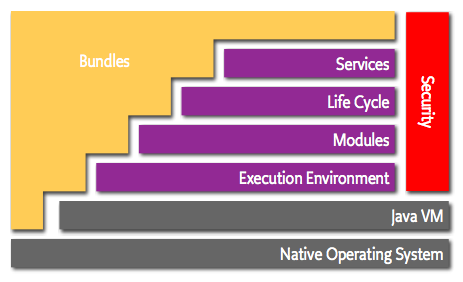
\includegraphics[width=0.8\textwidth]{graphics/OSGI.png}
	\caption{OSGI Layers \cite{noauthor_osgi_nodate} }	
	\label{pic: OSGILayers}
\end{figure} 

Bundles sind Module sie sind die kleinste Einheit der Modularisierung. Ein Bundle ist eine JAR-Datei mit zusätzlichen Meta-Informationen.\\
\\
In den Meta-Informationen sind Bundlesabhängigkeits Informationen. Ein Bundle kann von einem andern Bundel oder von einem Paket abhängig sein.\\
\\
Die OSGi-Runtime verwendet die Informationen über die Abhängigkeiten, um die Bundles zu verdrahten und versteckt alles in dieser JAR, sofern es nicht explizit exportiert wird. Die Abhängigkeiten zu den Java-Standardbibliotheken werden durch den Bundle-Header verwaltet, so dass es nicht notwendig ist, die Java-Kernpakete zu importieren.\\
\\
Bundles werden oft zur Registrierung und zum Konsum von Dienstleistungen verwendet.\\
\\
Die Bundles können in Laufzeit installiert, deinstalliert und geändert werden. Die Spezifikationen der OSGI Architektur also Abhängigkeiten und der Mechanismus wird mit Hilfe des Lebenszykluskonzepts erreicht. Der Rahmen führt verschiedene Zustände ein und regelt wie sich die vom Bundle exportierten Pakete und Dienste auswirken. 

 \begin{figure}[H]
	\centering
	\includegraphics[width=0.5\textwidth]{graphics/BundleState.png}
	\caption{Bundle State Diagramm \cite{noauthor_osgi_nodate}} 	
	\label{pic: BundleState}
\end{figure} 

In diesem Diagramm ist ersichtlich, dass Bundles während des Ausführens nicht geändert werden können, sonnst aber jederzeit.

\subsubsection{JAR}
\subsubsection{Übersicht Kommunikation Verbindungen}
Die Kommunikation zwischen den Komponenten geschieht mittels Event Bus. Alle nicht Status bezogenen Bundels informieren darüber andere Bundles über den Status von Events. Über diesen Bus Kommunizieren alle Binding mit einem phsikalischen Link zur realen Hardware. Mit dem Events werden auf asynchrone weise in diesem Bus veröffentlicht, durch den EventSubscriber definierte Callback-Schnittstellen werden diese zur entsprechender Funktion vorgesehenen Events wiederum Empfangen. Der EventSubsciber ist als OSGI Dienst registriert \cite{noauthor_event_nodate}.

  \begin{figure}[H]
 	\centering
 	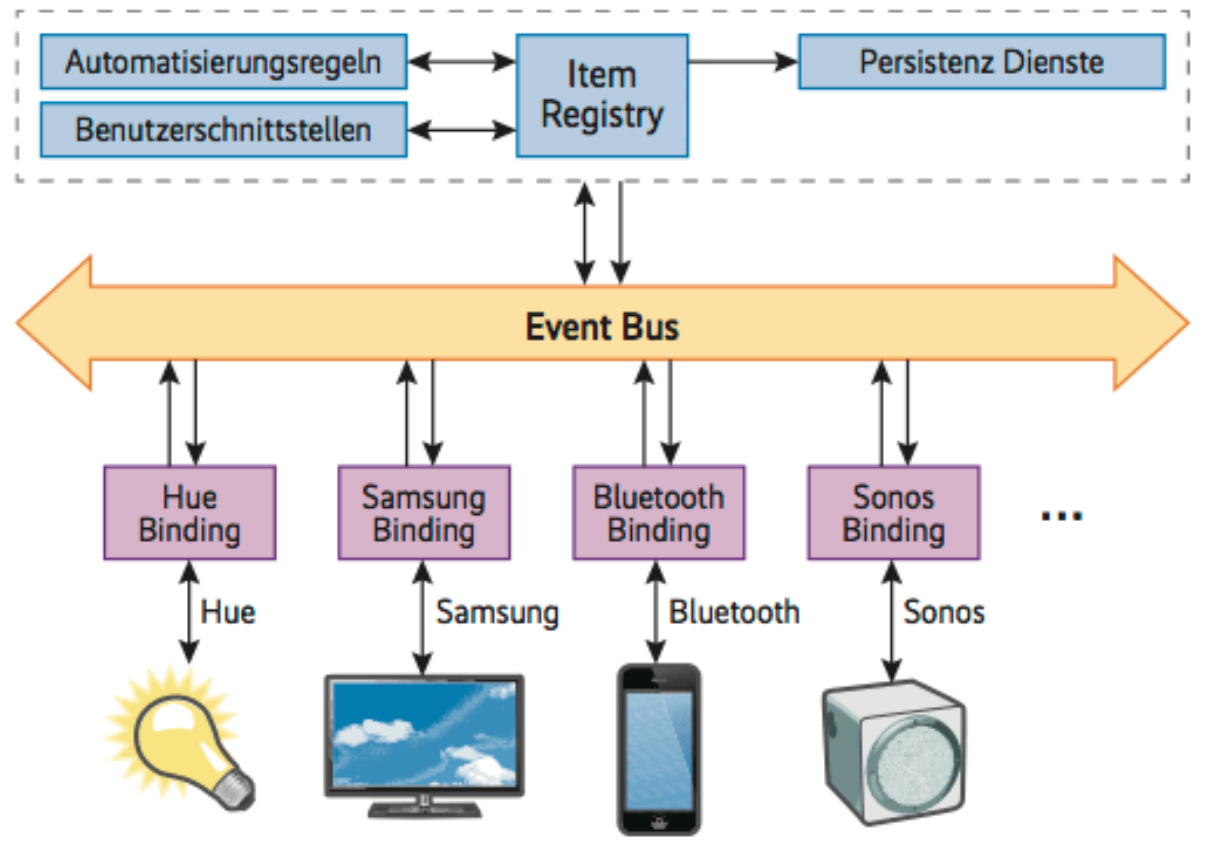
\includegraphics[width=0.8\textwidth]{graphics/Eventbus.PNG}
 	\caption{Eventbus Openhab \cite{noauthor_durchbruch_nodate } }	
 	\label{pic: Eventbus}
 \end{figure} 
 
 In der Abbildung \ref{pic: Eventbus} ist der Eventbus dargestellt verschiedene Bindings mit Hardwarekomponenten von verschiedenen Smarthome Lösungen empfangen, die für sie vorgesehene Events